\documentclass[tikz,border=6pt]{standalone}
\usepackage{amsmath,amssymb}
\usepackage{xcolor}
\definecolor{accent}{HTML}{A13D2C}
\definecolor{accent2}{HTML}{2B5F6B}
\definecolor{muted}{HTML}{5A564F}
\definecolor{panel}{HTML}{F8F6F0}
\definecolor{linecol}{HTML}{D8D2C4}
\definecolor{astroblue}{HTML}{1B4F72}
\definecolor{ink}{HTML}{1E1C1A}
\usetikzlibrary{calc,arrows.meta}
\usepackage{pgfplots}\pgfplotsset{compat=1.18}
\usepackage[T1]{fontenc}\usepackage{newpxtext,newpxmath}  % same fonts as the notes
\begin{document}
% Schematic opacity of the Earth's atmosphere at the ground (high, dry site) against wavelength, with the band
% names and frequencies above and the cause of the absorption in each range below. Band edges follow
% chapter 5 section 'Windows on the Universe': ozone edge 300 nm, plasma frequency ~10 MHz (30 m),
% infrared windows J H K L M N, water vapour bands 1.4, 1.9, 2.7, 6.3 um, CO2 4.3, 15 um, O2 60 and 118 GHz,
% H2O 22 and 183 GHz. Heights between the edges are schematic. x = log10(lambda / m).
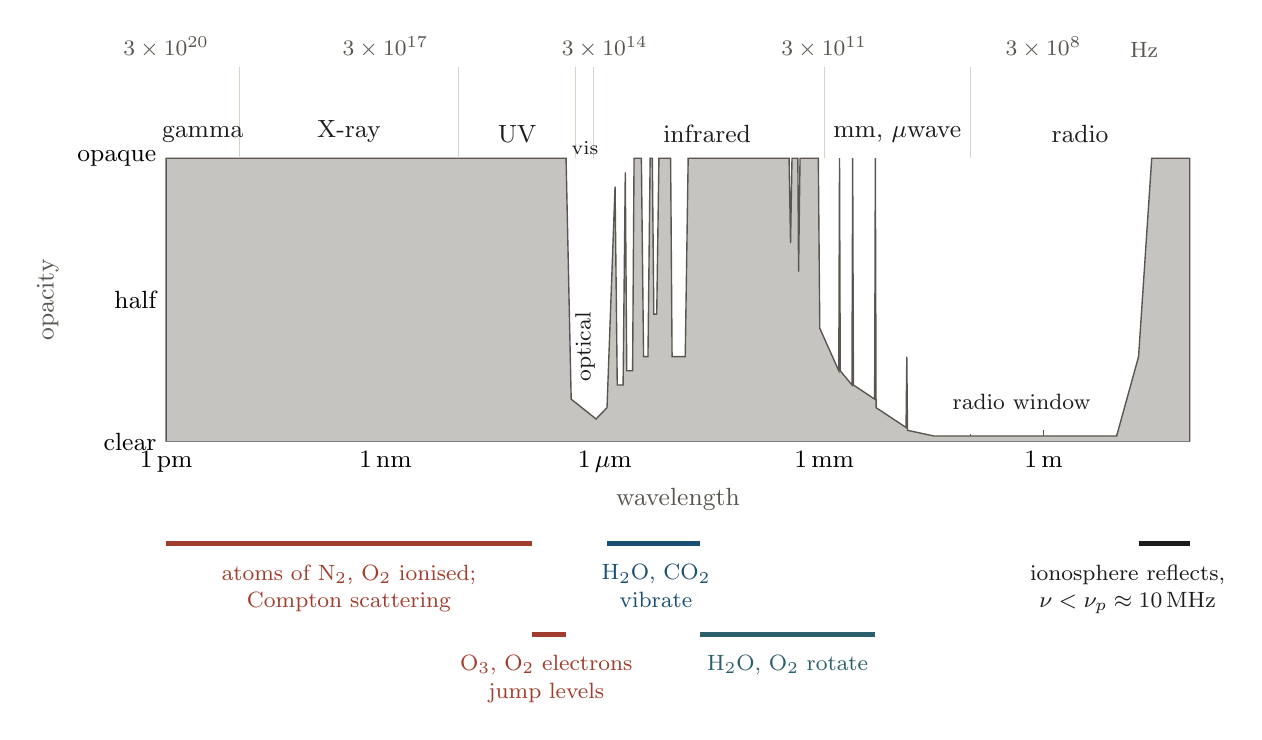
\begin{tikzpicture}[font=\small]
  \begin{axis}[width=13cm, height=3.6cm, scale only axis, axis lines*=left,
      xmin=-12, xmax=2, ymin=0, ymax=1, clip=false,
      xtick={-12,-9,-6,-3,0}, xticklabels={1\,pm,1\,nm,1\,$\mu$m,1\,mm,1\,m},
      minor xtick={-11,-10,-8,-7,-5,-4,-2,-1,1,2},
      ytick={0,0.5,1}, yticklabels={clear,half,opaque},
      tick style={muted}, every axis label/.style={text=muted},
      xlabel={wavelength}, ylabel={opacity}, xlabel style={at={(axis description cs:0.5,-0.13)}}]
    \addplot[fill=muted!35, draw=muted, line width=0.5pt] coordinates {
      (-12,0) (-12,1) (-6.53,1) (-6.46,0.15) (-6.12,0.08)
      (-5.97,0.12) (-5.86,0.9) (-5.83,0.2) (-5.75,0.2) (-5.72,0.95) (-5.70,0.25) (-5.62,0.25)
      (-5.60,1) (-5.50,1) (-5.47,0.3) (-5.41,0.3) (-5.38,1) (-5.35,1) (-5.33,0.45) (-5.29,0.45)
      (-5.26,1) (-5.10,1) (-5.08,0.3) (-4.90,0.3) (-4.86,1)
      (-3.48,1) (-3.46,0.7) (-3.44,1) (-3.36,1) (-3.35,0.6) (-3.33,1) (-3.08,1) (-3.06,0.4)
      (-2.80,0.25) (-2.79,1) (-2.78,0.25) (-2.62,0.2) (-2.61,1) (-2.60,0.2) (-2.31,0.15) (-2.30,1) (-2.29,0.12)
      (-1.88,0.05) (-1.87,0.3) (-1.86,0.04) (-1.5,0.02) (1.0,0.02) (1.3,0.3) (1.48,1) (2,1) (2,0) };
    % band names and frequencies above
    \pgfplotsinvokeforeach{-11,-8,-6.4,-6.15,-3,-1}{\draw[linecol] (axis cs:#1,1) -- (axis cs:#1,1.32);}
    \node[ink, anchor=south] at (axis cs:-11.5,1.02) {gamma};
    \node[ink, anchor=south] at (axis cs:-9.5,1.02) {X-ray};
    \node[ink, anchor=south] at (axis cs:-7.2,1.02) {UV};
    \node[ink, anchor=south] at (axis cs:-4.6,1.02) {infrared};
    \node[ink, anchor=south] at (axis cs:-2,1.02) {mm, $\mu$wave};
    \node[ink, anchor=south] at (axis cs:0.5,1.02) {radio};
    \node[ink, anchor=south, inner sep=1pt] at (axis cs:-6.27,1.0) {\scriptsize vis};
    \node[muted, anchor=south] at (axis cs:-12,1.32) {\footnotesize $3\times10^{20}$};
    \node[muted, anchor=south] at (axis cs:-9,1.32) {\footnotesize $3\times10^{17}$};
    \node[muted, anchor=south] at (axis cs:-6,1.32) {\footnotesize $3\times10^{14}$};
    \node[muted, anchor=south] at (axis cs:-3,1.32) {\footnotesize $3\times10^{11}$};
    \node[muted, anchor=south] at (axis cs:0,1.32) {\footnotesize $3\times10^{8}$};
    \node[muted, anchor=south west] at (axis cs:1.05,1.32) {\footnotesize Hz};
    % windows named inside the clear parts
    \node[ink, rotate=90, anchor=west, inner sep=1pt] at (axis cs:-6.27,0.2) {\footnotesize optical};
    \node[ink, anchor=south] at (axis cs:-0.3,0.08) {\footnotesize radio window};
    % causes, as bars below the axis
    \pgfmathsetmacro{\ya}{-0.36}\pgfmathsetmacro{\yb}{-0.68}
    \draw[accent, line width=2pt] (axis cs:-12,\ya) -- (axis cs:-7,\ya);
    \node[accent, anchor=north, align=center] at (axis cs:-9.5,\ya-0.04) {\footnotesize atoms of $\mathrm N_2$, $\mathrm O_2$ ionised;\\[-1pt]\footnotesize Compton scattering};
    \draw[accent, line width=2pt] (axis cs:-7,\yb) -- (axis cs:-6.53,\yb);
    \node[accent, anchor=north, align=center] at (axis cs:-6.8,\yb-0.04) {\footnotesize $\mathrm O_3$, $\mathrm O_2$ electrons\\[-1pt]\footnotesize jump levels};
    \draw[astroblue, line width=2pt] (axis cs:-5.97,\ya) -- (axis cs:-4.7,\ya);
    \node[astroblue, anchor=north, align=center] at (axis cs:-5.3,\ya-0.04) {\footnotesize $\mathrm H_2\mathrm O$, $\mathrm{CO}_2$\\[-1pt]\footnotesize vibrate};
    \draw[accent2, line width=2pt] (axis cs:-4.7,\yb) -- (axis cs:-2.3,\yb);
    \node[accent2, anchor=north, align=center] at (axis cs:-3.5,\yb-0.04) {\footnotesize $\mathrm H_2\mathrm O$, $\mathrm O_2$ rotate};
    \draw[ink, line width=2pt] (axis cs:1.3,\ya) -- (axis cs:2,\ya);
    \node[ink, anchor=north, align=center] at (axis cs:1.15,\ya-0.04) {\footnotesize ionosphere reflects,\\[-1pt]\footnotesize $\nu<\nu_p\approx10\,$MHz};
  \end{axis}
\end{tikzpicture}
\end{document}
